\subsection{Grundlagen der Imperativen Programmierung}



\subsubsection{Von-Neumann-Architektur}

\begin{itemize}
	\item Ein Rechner besteht aus vier Komponenten/Bestandteilen:
	\begin{itemize}
		\item CPU (Central Processing Unit) - \textcolor{red}{\textbf{Steuerwerk}}
		\item Memory (Speicher/RAM)
		\item Ein/Ausgabe (I/O)
		\item BUS - verbindet alle Komponenten
	\end{itemize}
\end{itemize}

\begin{figure}[h!] % Option h! = hier, wenn möglich
	\centering %Bild zentrieren
	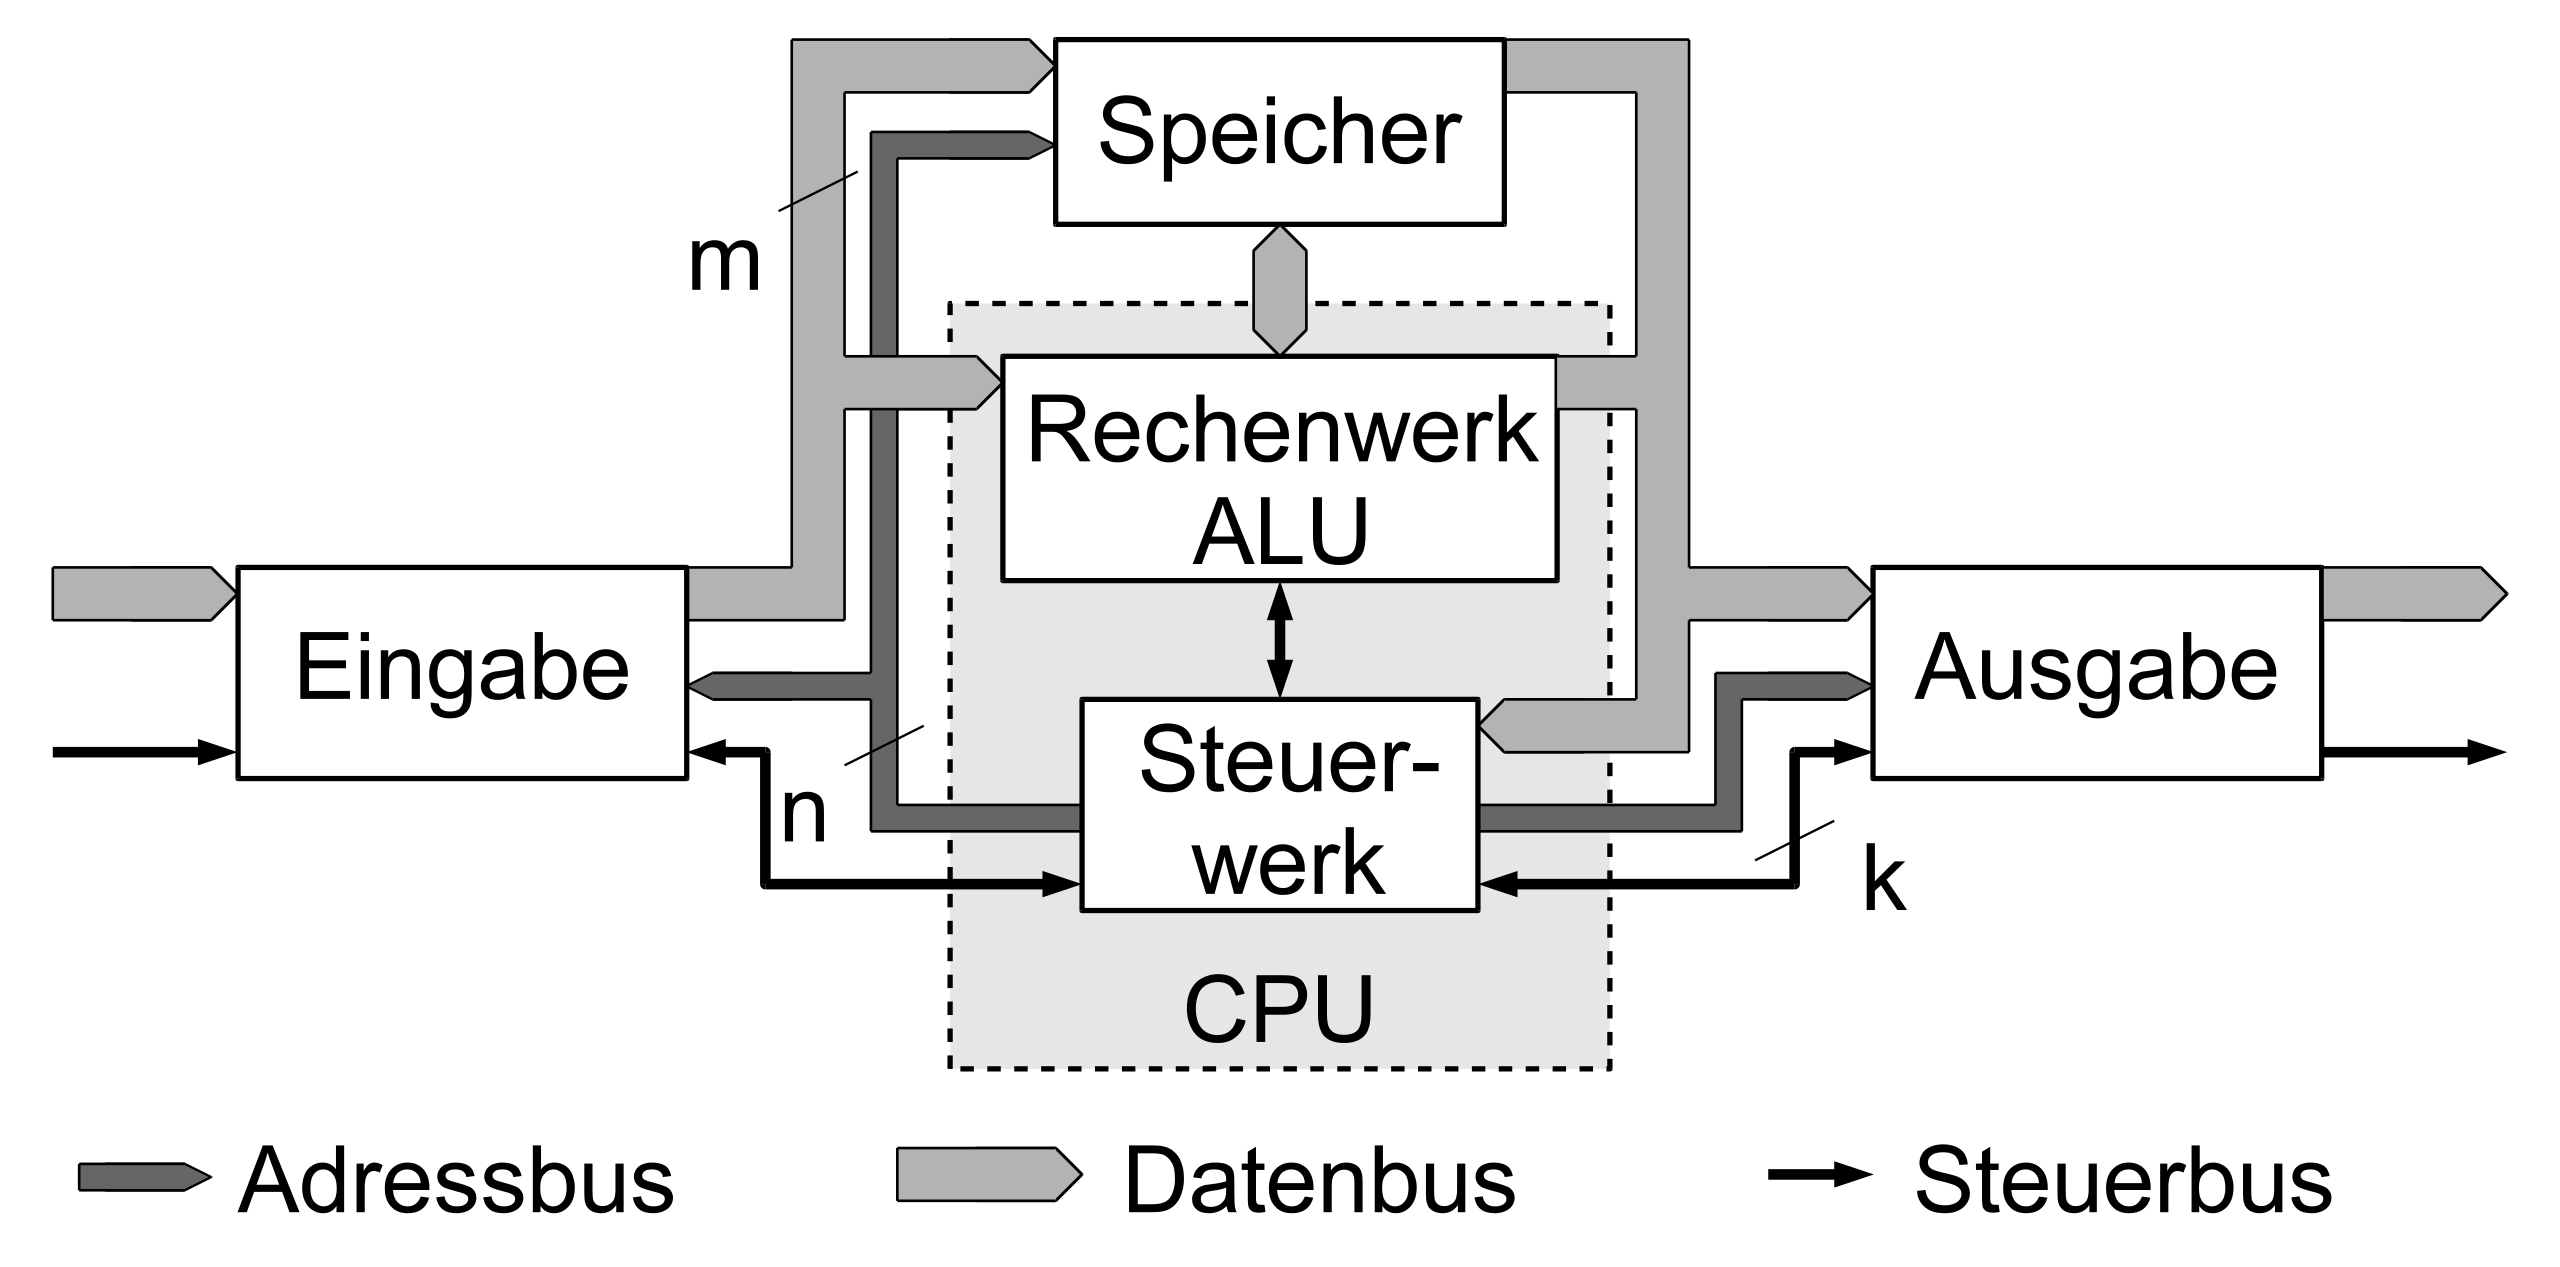
\includegraphics[width=0.8\textwidth]{Bilder/Von-Neumann-Architektur}
	\caption{Bildunterschrift}
	\label{fig:Bild} % Verweis mit \ref möglich
\end{figure}

\begin{itemize}

	\item CPU (Central Processing Unit)
	
	\begin{itemize}
		
		\item CU (Control Unit)
		
		\begin{itemize}
			\item Koordiniert die Ausführung von Befehle
		\end{itemize}
		
		\item ALU (Arithmetic Logical Unit) - \textcolor{red}{\textbf{Rechenwerk}}
		\begin{itemize}
			\item Das sind die Schaltkreise um die wirklichen Berechnung durchzuführen
		\end{itemize}
		
		\item Clock (Taktgeber)
		\begin{itemize}
			\item Sendet regelmäßig impulse aus, um einen Takt vorzugeben
			\item Ein Quwarz der mit Strom (CEmos Batterie) in Schwingung versetzt wird
		\end{itemize}
		
		\item PC ( Program counter - Programmzähler )
		\begin{itemize}
			\item Adressiert diejenige Zelle im Hauptspeicher (Memory) bei dem die nächste Anweisung beginnt
		\end{itemize}
	\end{itemize}
	
	\item Speicher (RAM)
	\begin{itemize}
		\item Speichert die Daten und Programme
		\item RAM (Random Access Memory)
		\begin{itemize}
			\item Speicher besteht aus Zellen
			\item Zellen sind durchnummeriert, z.B. von 0 bis n-1
			\item Alle Zellen sind gleich groß, zwischen 0 und x (Hardware abhängig)
			\item Jede Zelle speichert eine Zahl, repräsentiert in Bits
			\item 8 Bits/16 Bits/32 Bits/64 Bits - sind mögliche Variationen, jenachdem wie das System aufgebaut ist
		\end{itemize}
	\end{itemize}


	\item \textbf{Funktionalität} des Speichers: Lesen und Schreiben.
	\begin{itemize}
		\item Lese die Zelle 100 oder schreibe in die Zelle 100
		\item schreibe zahl z in Speicherzelle h
		\item wird in beliebiger Reihenfolge unterstützt
	\end{itemize}
	
	\item ROM (Read only Memory)
	
	\item Ein/Ausgabe (I/O)
	\begin{itemize}
		\item Sind Physikalische Geräte, die erlauben mit dem Computer von außerhalb zu Kommunizieren wie: Tastartur, Maus, Drucker, Kamera, Bildschirm, Netzwerkinterface, USB-Anschluss, ...usw.
	\end{itemize}
	
	\item BUS
	\begin{itemize}
		\item sind Kabel/Leitungen/Drähte, die alle Komponenten miteinander verbinden
	\end{itemize}
\end{itemize}

\subparagraph{\textbf{Funktionsweise}}
Solange der Rechner eingeschaltet ist, führt er die folgende Schritte immer wieder aus. \\
- FETCH - CU weißt den Memory über den Bus an, den Inhalt der Speicherzelle mit Adresse PC zu liefern \\
- DECODE - (Dekodiere/Interpretiere) CU schaut nach um welche Anweisung es sich handelt und holt gegebenenfalls weitere Bestandteile der Anweisung aus dem Memory \\
- EXECUTE - CU sorgt dafür, das Anweisung ausgeführt wird, indem sie die andere Komponente Koordiniert \\
- Aktualisiere PC \\
- REPEAT - Wiederholt den Durchlauf \\

\subsubsection{Programmiersprachen}

\subsubsection{Ausdrücke}

\subsubsection{Imperative Programmierung}

\subsection{Datentypen und Variablen}

\subsubsection{Primitive Datentypen}

\subsubsection{Zusammengesetzte Datentypen}

\subsubsection{Darstellung von Daten?}

\subsubsection{Die fünf Facetten von Variablen}

\subsection{Unterprogramme und Funktionen}

\subsubsection{Fundamentale Unterprogramme}

\subsubsection{Parameter Übergabe Strategien}

\subsubsection{Rekursion}

\subsubsection{Fünf schritte für die Implementierung von einer Funktion}

\subsubsection{Case Study ???}